\documentclass{article}
\setlength{\parskip}{5pt} % esp. entre parrafos
\setlength{\parindent}{0pt} % esp. al inicio de un parrafo
\usepackage{amsmath} % mates
\usepackage[sort&compress,numbers]{natbib} % referencias
\usepackage{url} % que las URLs se vean lindos
\usepackage[top=25mm,left=20mm,right=20mm,bottom=25mm]{geometry} % margenes
\usepackage{hyperref} % ligas de URLs
\usepackage{graphicx} % poner figuras
\usepackage[spanish]{babel} % otros idiomas
\usepackage[utf8]{inputenc} % alparecer son los acentos
\documentclass[12pt,letterpaper]{article}
\usepackage[utf8]{inputenc}
\usepackage{tikz}
\usetikzlibrary{trees}
\usepackage[spanish, es-nodecimaldot]{babel}
\usepackage{color}
\usepackage{algorithm}
\usepackage[noend]{algpseudocode}
\renewcommand{\algorithmicrequire}{\textbf{Entrada:}}
\renewcommand{\algorithmicensure}{\textbf{Salida:}}
\usepackage{subcaption}
\usepackage{amsfonts}
\usepackage{hyperref}
 \hypersetup{
     colorlinks=true,
     linkcolor=blue,
     filecolor=blue,
     citecolor = blue,      
     urlcolor=cyan,
     }
\usepackage{amssymb}
\usepackage{listings}
\usepackage{color}
\author{I E G} % author
\title{Práctica 11 : Frentes de Pareto} % titulo
\date{\today}

\begin{document} % inicia contenido

\maketitle % cabecera

\begin{abstract} % resumen
En esta práctica la se utiliza la optimización multicriterio \cite{elis11} donde a un mismo conjunto de variables se le asignan valores de forma que optimicen dos o más funciones objetivo sin que una mejora empeore a la otra figura \ref{figura1}. El objetivo de esta practica es observar el porcentaje de soluciones que pertenecen al frente al ir incrementando la cantidad de funciones objetivo para $k \in \{2,3,\ldots,9\}$ graficando con diagramas de violín que sean combinados con diagramas de caja bigote, verificando las diferencias observadas estadísticamente significativas.



\begin{figure} [h!]% figura
    \centering
    \includegraphics[width=129mm]{Fig1.png} % archivo
    \caption{Ejemplo bidimencional de frente de Pareto.}
    \label{figura1}
\end{figure}

\end{abstract}


\section{Desarrollo}




Se utiliza el lenguaje de programación Python 3.9.6 para la generación del código previamente reportado en \cite{elis11,denis11} primero se generan polinomios pseudo aleatorios y se determina si se va a minimizar o maximizar. Se determinan todas aquellas soluciones que dominan y a dicho conjunto de soluciones se le denomina frente de Pareto. Al código fuente de módica agregando dos ciclos for para las replicas que son 30 y para variar las funciones objetivo. El número de soluciones aleatorias es de 280.




\begin{lstlisting}
iteracion = 30 # cuantas iteraciones
porcentajes = []
for k in range(1, 10): # cuantas funciones objetivo

    for it in range(iteracion): 
        vc = 4
        md = 3
        tc = 5
        obj = [poli(md, vc, tc) for i in range(k)]
        minim = np.random.rand(k) > 0.5
        n = 280 # cuantas soluciones aleatorias
        sol = np.random.rand(n, vc)
        val = np.zeros((n, k))
        for i in range(n): # evaluamos las soluciones
            for j in range(k):
                val[i, j] = evaluate(obj[j], sol[i])
        sign = [1 + -2 * m for m in minim]
        
        no_dom = []
        for i in range(n):
            d = [domin_by(sign * val[i], sign * val[j]) for j in range(n)]
            no_dom.append(not np.any(d)) # si es cierto que ninguno es verdadero
        frente = val[no_dom, :]
        porcentaje = (len(frente)/n)*100
        porcentajes.append(porcentaje)
\end{lstlisting}

Finalmente se gráfica los porcentajes de cada función en grafica violín figura \fer{fig2}.  

\section{Experimento}
Para $k \in \{2,3,\ldots,9\}$ se grafica con diagramas de violín que sean combinados con diagramas de caja bigote, donde se observa en la figura \ref{fig2} que el porcentaje de las soluciones pertenecen al frente de Pareto para cada función se observa además con 6  es el 50 de porcentaje y para las funciones 7 o más el porcentaje es casi la totalidad del porcentaje como en el cuadro \ref{data}.
\begin{figure} [h!]% figura
    \centering
    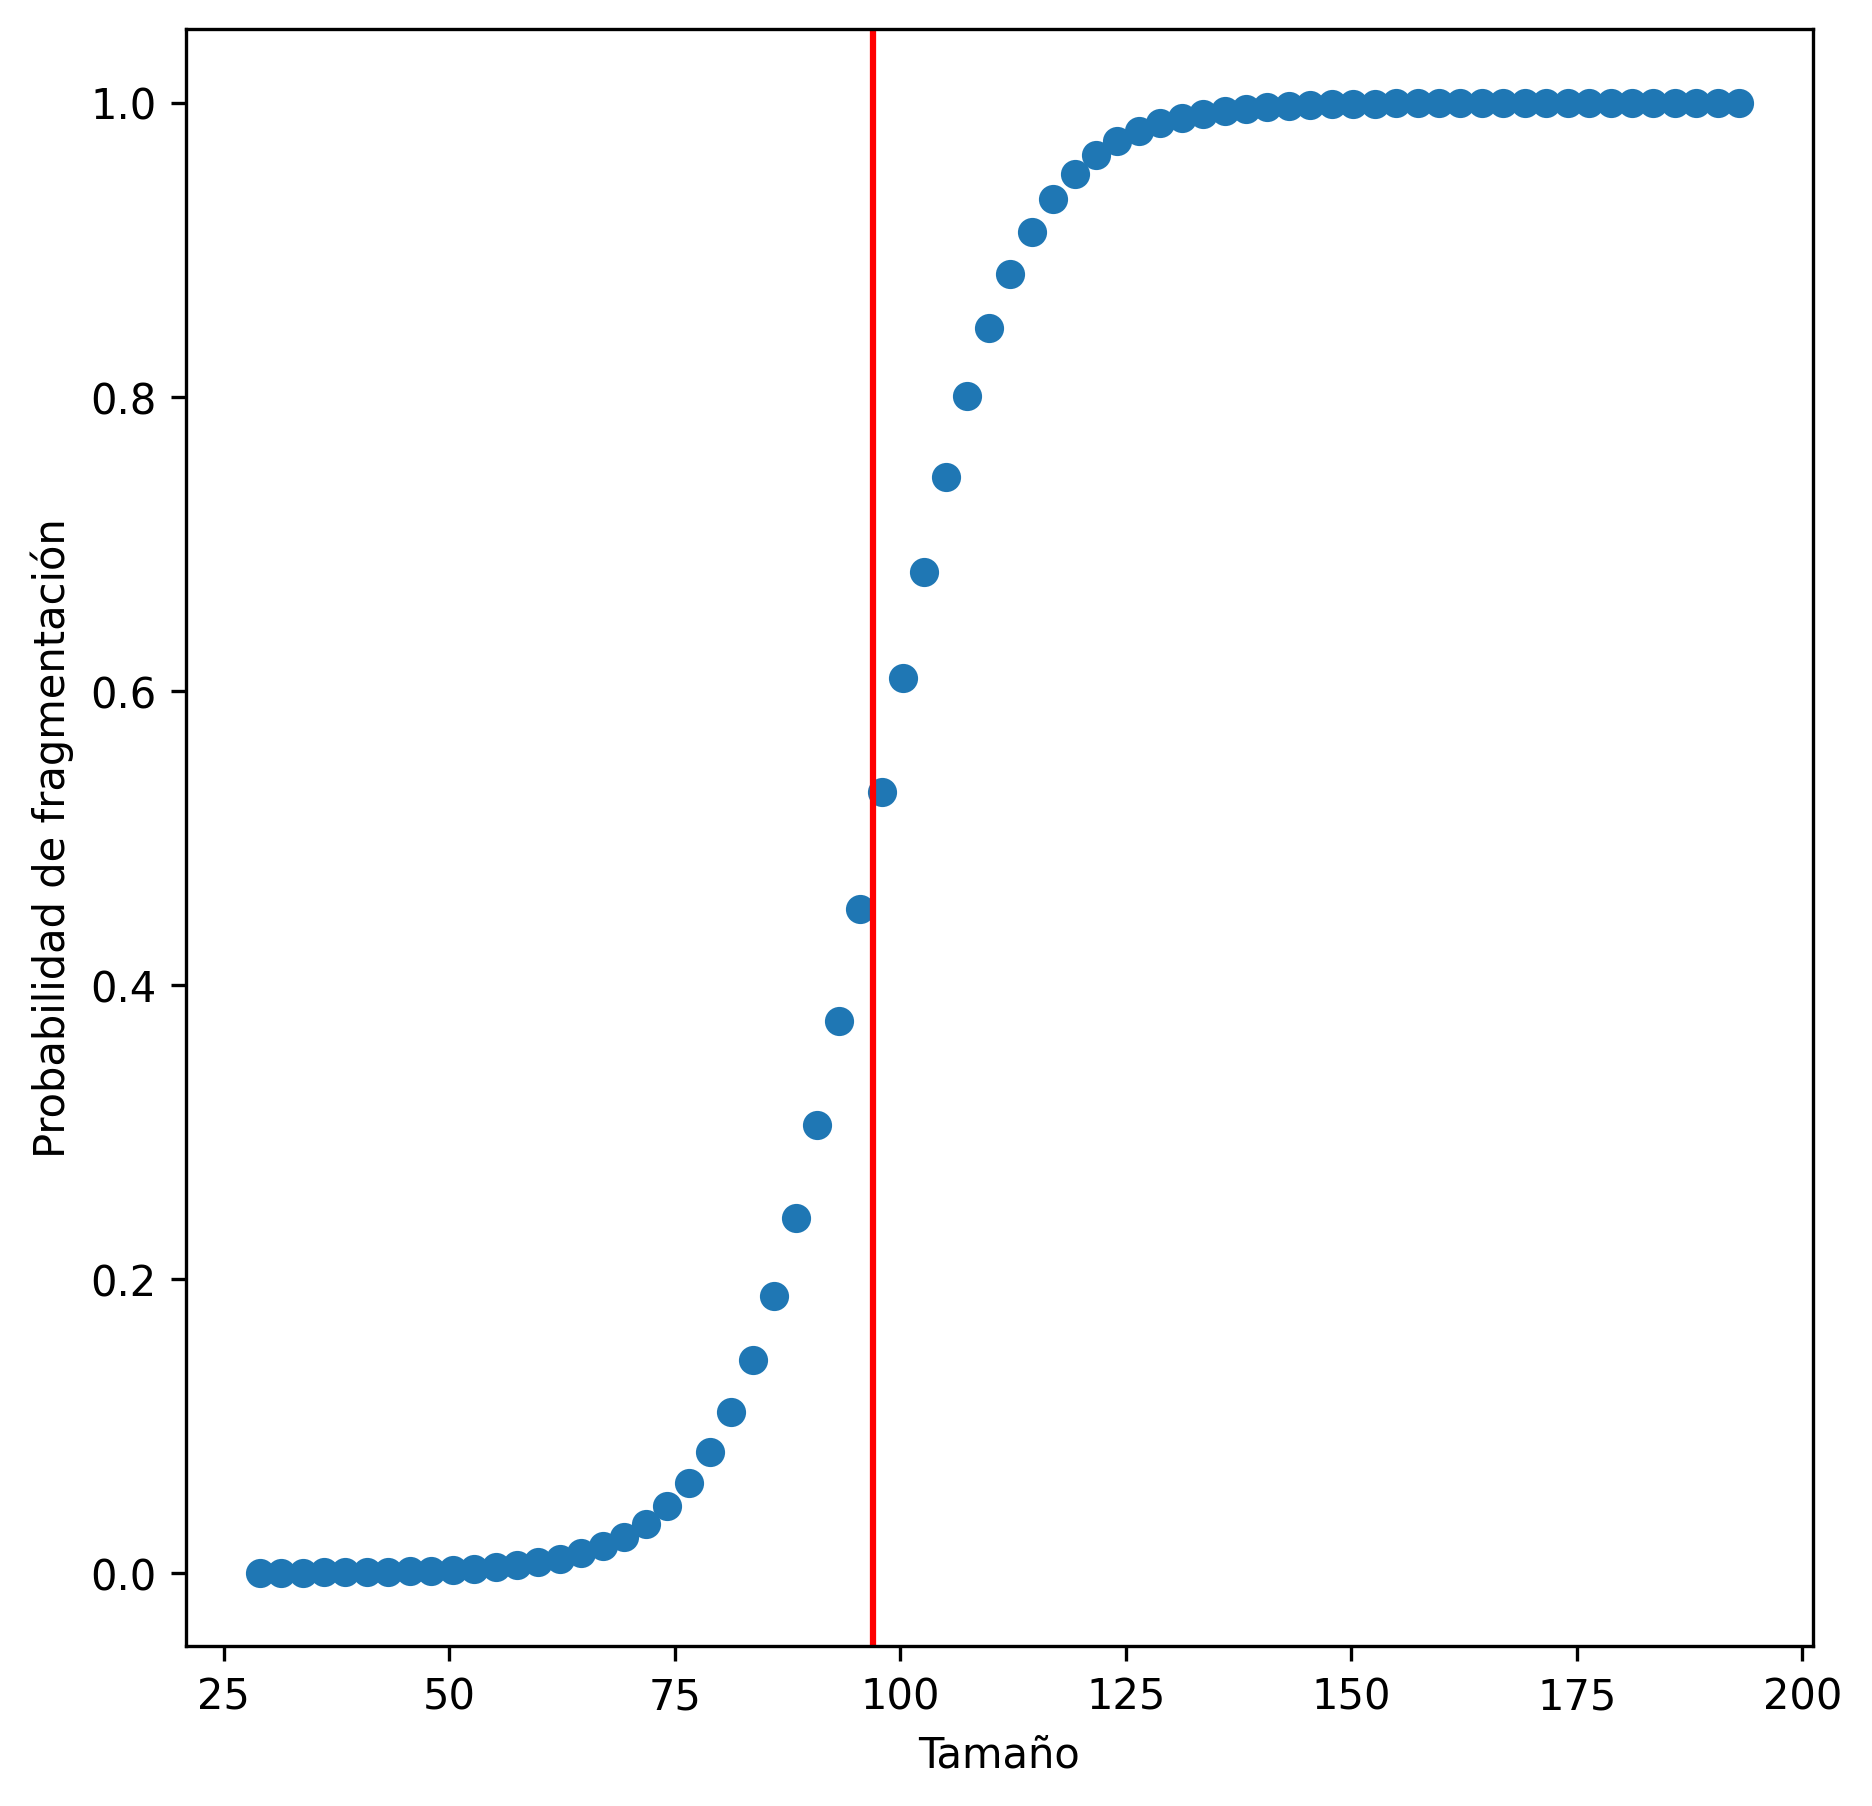
\includegraphics[width=129mm]{fig2.png} % archivo
    \caption{Gráficos de violín del porcentajes frente de Pareto.}
    \label{fig2}
\end{figure}

\begin{table} [h]
\centering
\caption{Porcentaje de los datos.}
\begin{tabular}{rr}
  \hline
Funciones & Porcentaje \\ 
  \hline
2 & 8.0 \\
3 & 24.0\\
4 & 1.0 \\
5 & 1.0 \\
6 & 57.0 \\
7 & 99.0 \\
8 & 99.5 \\
9 & 100.0\\
\hline
\end{tabular}
\label{data}
\end{table}
 
\section{Conclusiones} 

En conclusión, el porcentaje de soluciones de frente de Pareto no dominantes aumenta conforme se incrementa el número de funciones objetivo, para trabajo futuro y un estudio más profundo la hipótesis seria: mientras más funciones se agrega al sistema se puede llegar a una solución más perfecta.




\bibliography{bib}
\bibliographystyle{plainnat}

\end{document}